% Created by tikzDevice version 0.10.1 on 2017-12-03 20:41:44
% !TEX encoding = UTF-8 Unicode
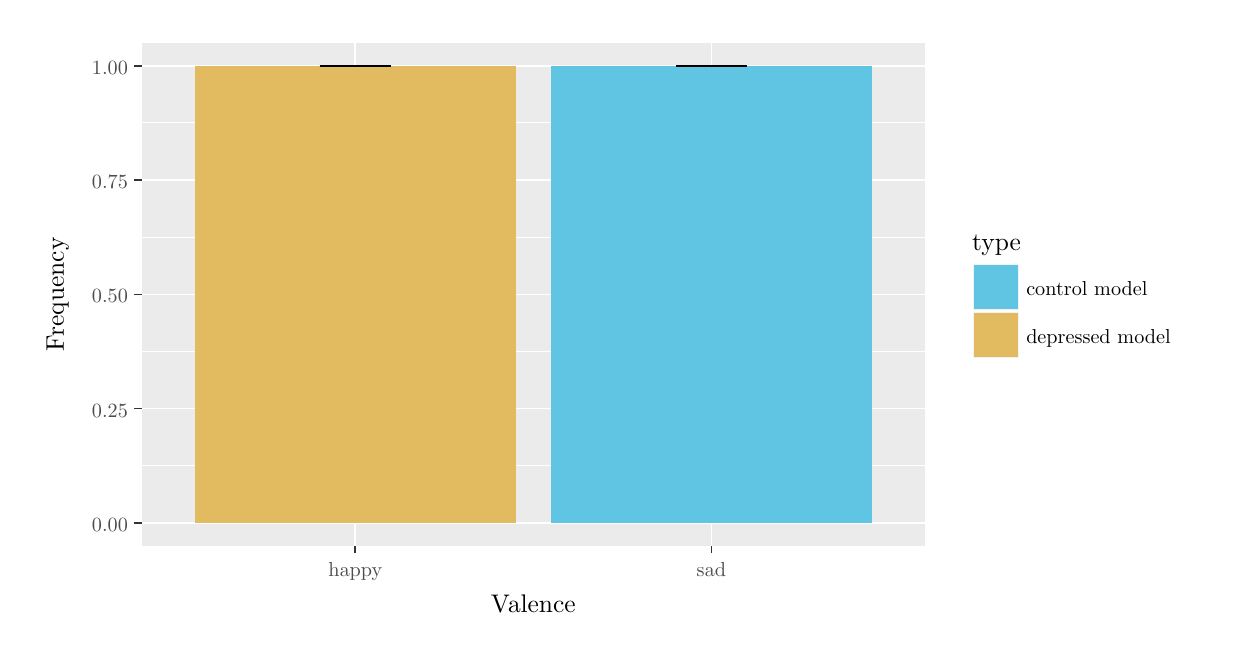
\begin{tikzpicture}[x=1pt,y=1pt]
\definecolor{fillColor}{RGB}{255,255,255}
\path[use as bounding box,fill=fillColor,fill opacity=0.00] (0,0) rectangle (433.62,216.81);
\begin{scope}
\path[clip] (  0.00,  0.00) rectangle (433.62,216.81);
\definecolor{drawColor}{RGB}{255,255,255}
\definecolor{fillColor}{RGB}{255,255,255}

\path[draw=drawColor,line width= 0.6pt,line join=round,line cap=round,fill=fillColor] (  0.00,  0.00) rectangle (433.62,216.81);
\end{scope}
\begin{scope}
\path[clip] ( 41.17, 29.59) rectangle (324.25,211.31);
\definecolor{fillColor}{gray}{0.92}

\path[fill=fillColor] ( 41.17, 29.59) rectangle (324.25,211.31);
\definecolor{drawColor}{RGB}{255,255,255}

\path[draw=drawColor,line width= 0.3pt,line join=round] ( 41.17, 58.50) --
	(324.25, 58.50);

\path[draw=drawColor,line width= 0.3pt,line join=round] ( 41.17, 99.80) --
	(324.25, 99.80);

\path[draw=drawColor,line width= 0.3pt,line join=round] ( 41.17,141.10) --
	(324.25,141.10);

\path[draw=drawColor,line width= 0.3pt,line join=round] ( 41.17,182.40) --
	(324.25,182.40);

\path[draw=drawColor,line width= 0.6pt,line join=round] ( 41.17, 37.85) --
	(324.25, 37.85);

\path[draw=drawColor,line width= 0.6pt,line join=round] ( 41.17, 79.15) --
	(324.25, 79.15);

\path[draw=drawColor,line width= 0.6pt,line join=round] ( 41.17,120.45) --
	(324.25,120.45);

\path[draw=drawColor,line width= 0.6pt,line join=round] ( 41.17,161.75) --
	(324.25,161.75);

\path[draw=drawColor,line width= 0.6pt,line join=round] ( 41.17,203.05) --
	(324.25,203.05);

\path[draw=drawColor,line width= 0.6pt,line join=round] (118.38, 29.59) --
	(118.38,211.31);

\path[draw=drawColor,line width= 0.6pt,line join=round] (247.05, 29.59) --
	(247.05,211.31);
\definecolor{fillColor}{RGB}{226,186,95}

\path[fill=fillColor] ( 60.47, 37.85) rectangle (176.28,203.05);
\definecolor{fillColor}{RGB}{95,197,226}

\path[fill=fillColor] (189.15, 37.85) rectangle (304.95,203.05);
\definecolor{drawColor}{RGB}{0,0,0}

\path[draw=drawColor,line width= 0.6pt,line join=round] (105.51,203.05) --
	(131.24,203.05);

\path[draw=drawColor,line width= 0.6pt,line join=round] (118.38,203.05) --
	(118.38,203.05);

\path[draw=drawColor,line width= 0.6pt,line join=round] (105.51,203.05) --
	(131.24,203.05);

\path[draw=drawColor,line width= 0.6pt,line join=round] (234.18,203.05) --
	(259.92,203.05);

\path[draw=drawColor,line width= 0.6pt,line join=round] (247.05,203.05) --
	(247.05,203.05);

\path[draw=drawColor,line width= 0.6pt,line join=round] (234.18,203.05) --
	(259.92,203.05);
\end{scope}
\begin{scope}
\path[clip] (  0.00,  0.00) rectangle (433.62,216.81);
\definecolor{drawColor}{gray}{0.30}

\node[text=drawColor,anchor=base east,inner sep=0pt, outer sep=0pt, scale=  0.73] at ( 36.22, 34.82) {0.00};

\node[text=drawColor,anchor=base east,inner sep=0pt, outer sep=0pt, scale=  0.73] at ( 36.22, 76.12) {0.25};

\node[text=drawColor,anchor=base east,inner sep=0pt, outer sep=0pt, scale=  0.73] at ( 36.22,117.42) {0.50};

\node[text=drawColor,anchor=base east,inner sep=0pt, outer sep=0pt, scale=  0.73] at ( 36.22,158.72) {0.75};

\node[text=drawColor,anchor=base east,inner sep=0pt, outer sep=0pt, scale=  0.73] at ( 36.22,200.02) {1.00};
\end{scope}
\begin{scope}
\path[clip] (  0.00,  0.00) rectangle (433.62,216.81);
\definecolor{drawColor}{gray}{0.20}

\path[draw=drawColor,line width= 0.6pt,line join=round] ( 38.42, 37.85) --
	( 41.17, 37.85);

\path[draw=drawColor,line width= 0.6pt,line join=round] ( 38.42, 79.15) --
	( 41.17, 79.15);

\path[draw=drawColor,line width= 0.6pt,line join=round] ( 38.42,120.45) --
	( 41.17,120.45);

\path[draw=drawColor,line width= 0.6pt,line join=round] ( 38.42,161.75) --
	( 41.17,161.75);

\path[draw=drawColor,line width= 0.6pt,line join=round] ( 38.42,203.05) --
	( 41.17,203.05);
\end{scope}
\begin{scope}
\path[clip] (  0.00,  0.00) rectangle (433.62,216.81);
\definecolor{drawColor}{gray}{0.20}

\path[draw=drawColor,line width= 0.6pt,line join=round] (118.38, 26.84) --
	(118.38, 29.59);

\path[draw=drawColor,line width= 0.6pt,line join=round] (247.05, 26.84) --
	(247.05, 29.59);
\end{scope}
\begin{scope}
\path[clip] (  0.00,  0.00) rectangle (433.62,216.81);
\definecolor{drawColor}{gray}{0.30}

\node[text=drawColor,anchor=base,inner sep=0pt, outer sep=0pt, scale=  0.73] at (118.38, 18.58) {happy};

\node[text=drawColor,anchor=base,inner sep=0pt, outer sep=0pt, scale=  0.73] at (247.05, 18.58) {sad};
\end{scope}
\begin{scope}
\path[clip] (  0.00,  0.00) rectangle (433.62,216.81);
\definecolor{drawColor}{RGB}{0,0,0}

\node[text=drawColor,anchor=base,inner sep=0pt, outer sep=0pt, scale=  0.92] at (182.71,  5.50) {Valence};
\end{scope}
\begin{scope}
\path[clip] (  0.00,  0.00) rectangle (433.62,216.81);
\definecolor{drawColor}{RGB}{0,0,0}

\node[text=drawColor,rotate= 90.00,anchor=base,inner sep=0pt, outer sep=0pt, scale=  0.92] at ( 13.08,120.45) {Frequency};
\end{scope}
\begin{scope}
\path[clip] (  0.00,  0.00) rectangle (433.62,216.81);
\definecolor{fillColor}{RGB}{255,255,255}

\path[fill=fillColor] (335.63, 91.46) rectangle (428.12,149.44);
\end{scope}
\begin{scope}
\path[clip] (  0.00,  0.00) rectangle (433.62,216.81);
\definecolor{drawColor}{RGB}{0,0,0}

\node[text=drawColor,anchor=base west,inner sep=0pt, outer sep=0pt, scale=  0.92] at (341.32,136.17) {type};
\end{scope}
\begin{scope}
\path[clip] (  0.00,  0.00) rectangle (433.62,216.81);
\definecolor{drawColor}{RGB}{255,255,255}
\definecolor{fillColor}{gray}{0.95}

\path[draw=drawColor,line width= 0.6pt,line join=round,line cap=round,fill=fillColor] (341.32,114.49) rectangle (358.67,131.84);
\end{scope}
\begin{scope}
\path[clip] (  0.00,  0.00) rectangle (433.62,216.81);
\definecolor{fillColor}{RGB}{95,197,226}

\path[fill=fillColor] (342.04,115.20) rectangle (357.96,131.13);
\end{scope}
\begin{scope}
\path[clip] (  0.00,  0.00) rectangle (433.62,216.81);
\definecolor{drawColor}{RGB}{255,255,255}
\definecolor{fillColor}{gray}{0.95}

\path[draw=drawColor,line width= 0.6pt,line join=round,line cap=round,fill=fillColor] (341.32, 97.15) rectangle (358.67,114.49);
\end{scope}
\begin{scope}
\path[clip] (  0.00,  0.00) rectangle (433.62,216.81);
\definecolor{fillColor}{RGB}{226,186,95}

\path[fill=fillColor] (342.04, 97.86) rectangle (357.96,113.78);
\end{scope}
\begin{scope}
\path[clip] (  0.00,  0.00) rectangle (433.62,216.81);
\definecolor{drawColor}{RGB}{0,0,0}

\node[text=drawColor,anchor=base west,inner sep=0pt, outer sep=0pt, scale=  0.73] at (360.84,120.13) {control model};
\end{scope}
\begin{scope}
\path[clip] (  0.00,  0.00) rectangle (433.62,216.81);
\definecolor{drawColor}{RGB}{0,0,0}

\node[text=drawColor,anchor=base west,inner sep=0pt, outer sep=0pt, scale=  0.73] at (360.84,102.79) {depressed model};
\end{scope}
\end{tikzpicture}
